Let $\tfone{\gL}$ and  $\tftwo{\gL}$ be languages in $\CoTtndn$, then there is a family of transformers $\{(\tfone{\TF})_n\}_{n \in \mathbb{N}}$ (resp. $\{(\tftwo{\TF})_n\}_{n \in \mathbb{N}}$) of embedding size $\tfone{d}(n)$ (resp. $\tftwo{d}(n)$) $\in O(d(n))$ that after $\tfone{T}(n)$ (resp. $\tftwo{T}(n)$) $\in T(n)$ steps of $\CoT$ computes $\tfone{\gL}$ (resp. $\tftwo{\gL}$).

We construct a family $\{\TF_n\}_{n \in \mathbb{N}}$ that computes $\tfone{\gL} \cup \tftwo{\gL}$.
It does it in $\tfone{T}(n) + \tftwo{T}(n) + 1 \in O(T(n))$ steps of $\CoT$ and it has embedding size $O(d(n))$.

The idea behind the construction is to run first one of the transformers, then run the other and finally compute the disjunction of both results as represented in Figure \ref{fig:or}.
The exact construction for $\TF$ is shown in appendix \ref{appendix:det-or}.


\begin{figure}[h!]
    \centering
    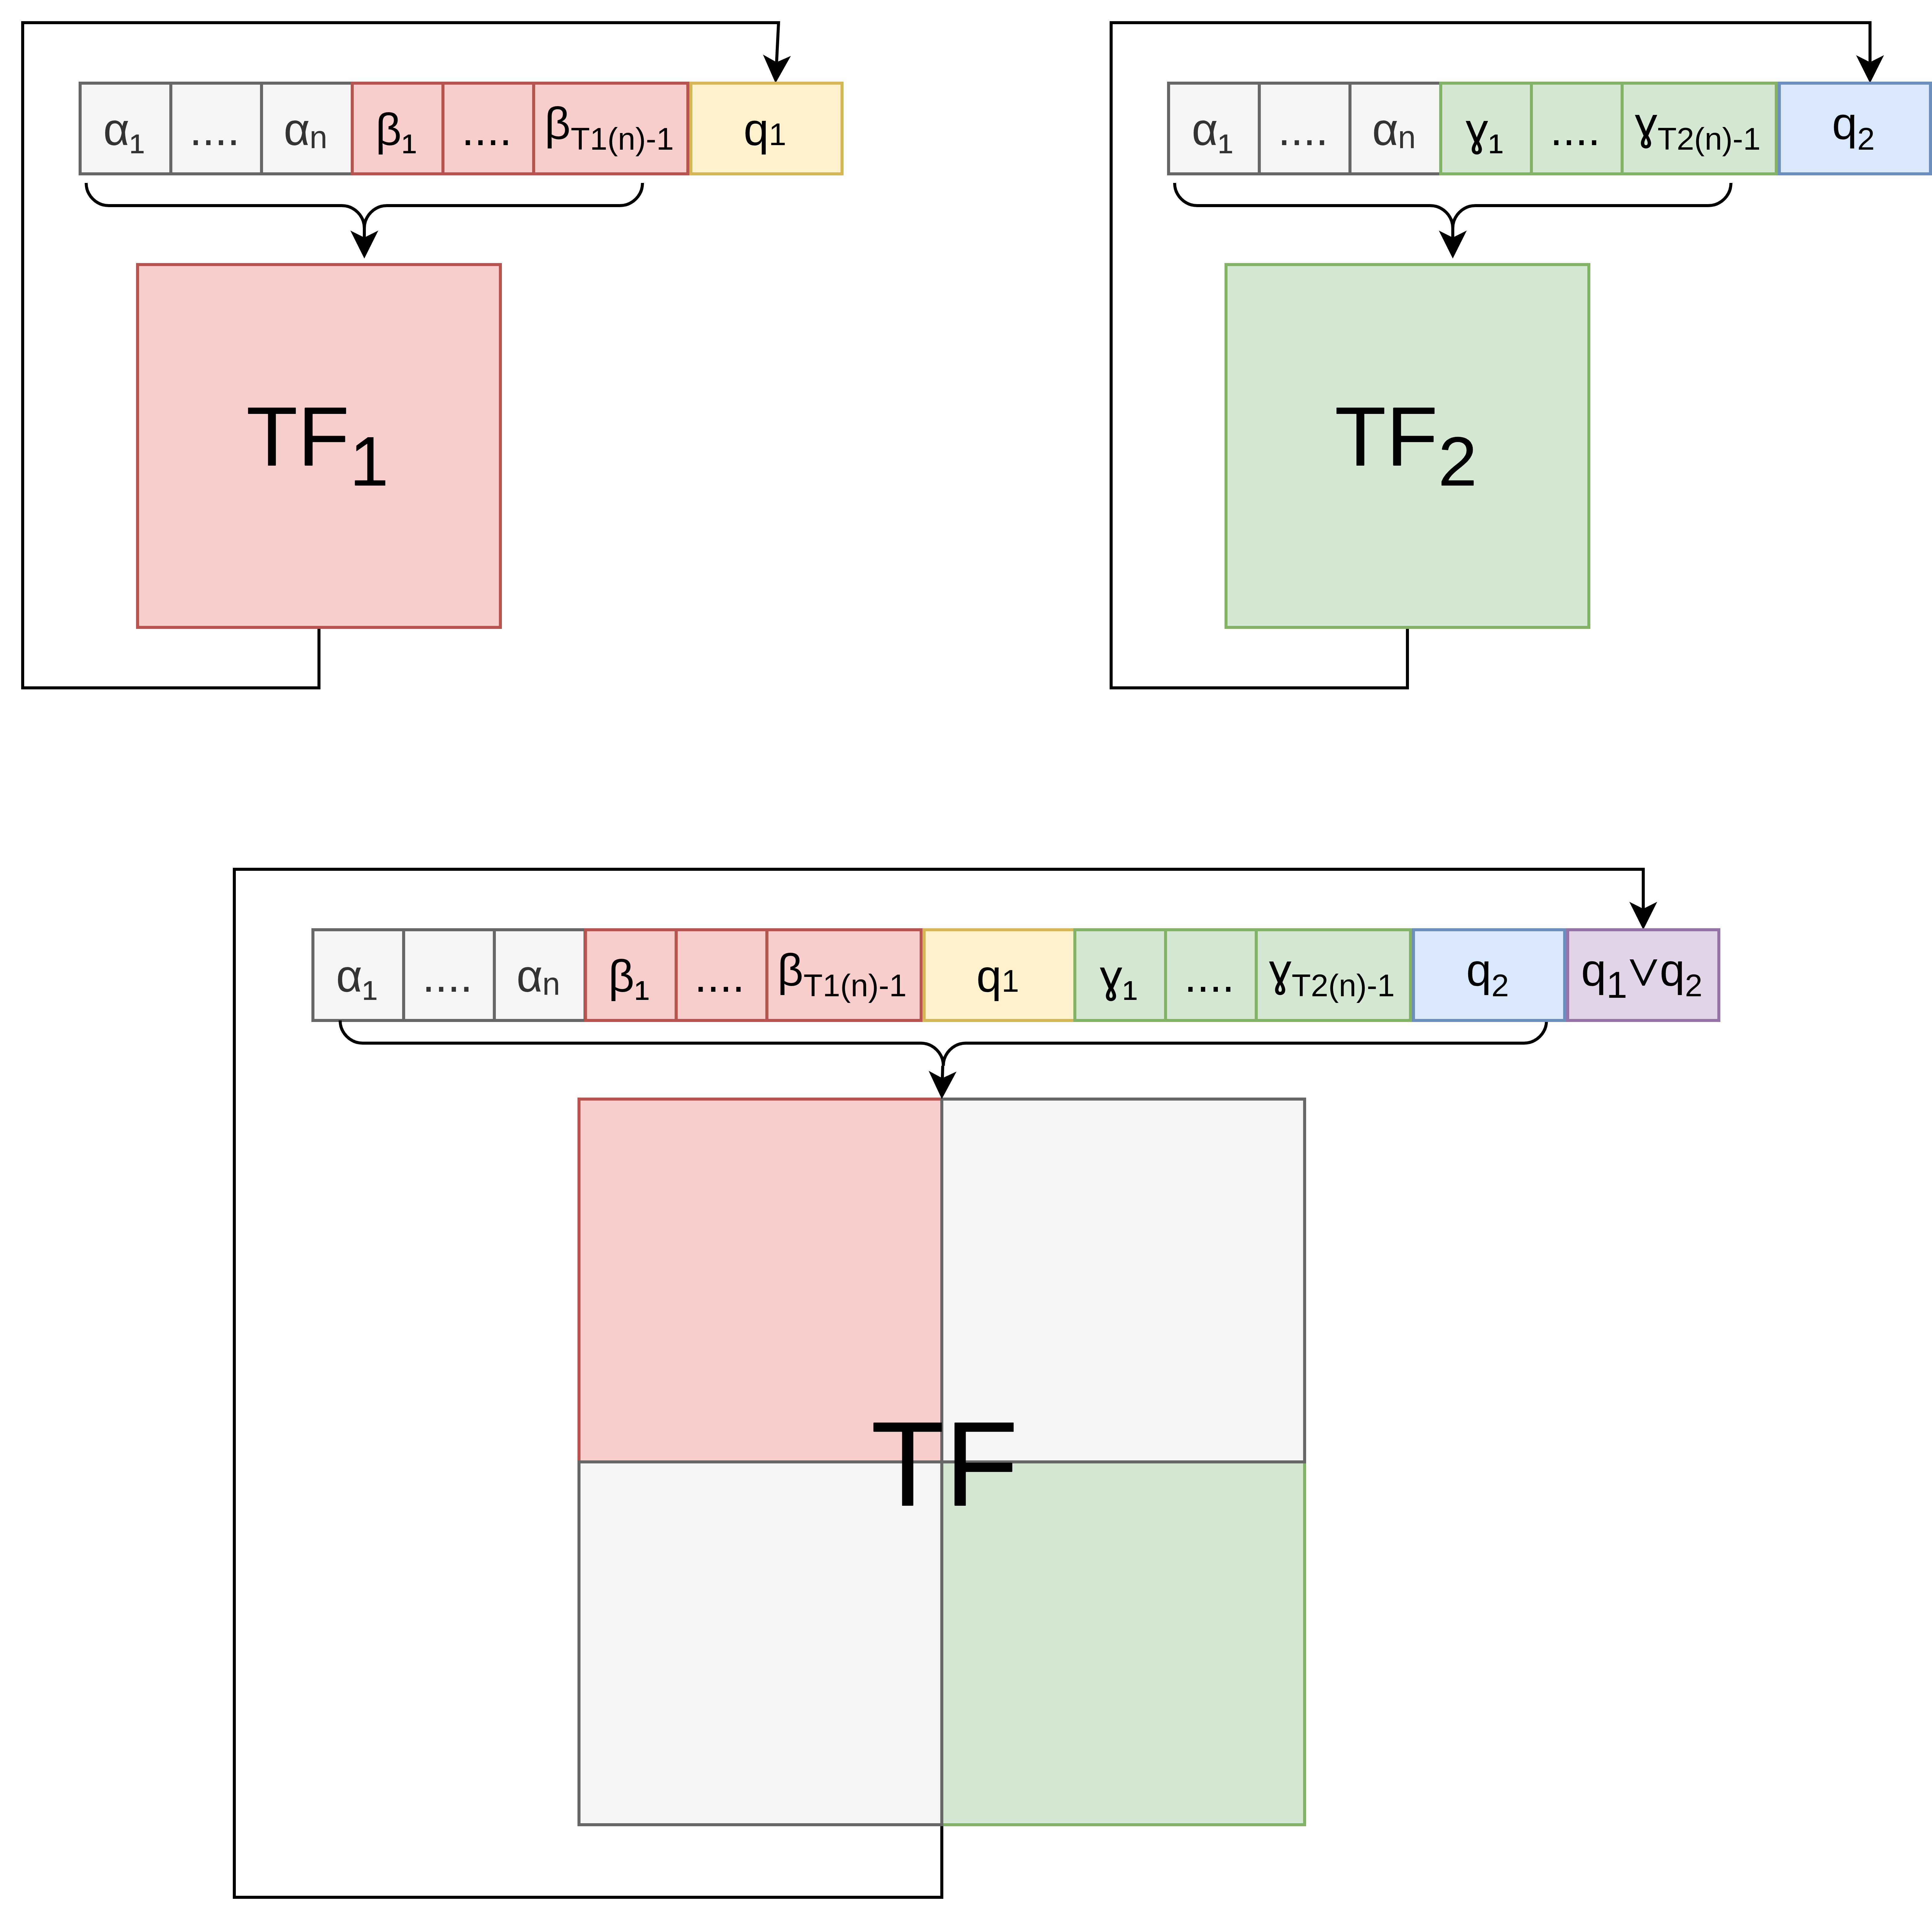
\includegraphics[width=0.5\textwidth]{chapters/diagrams/diagram-or.png}
    \caption{Visual representation of the construction for disjunction}
    \label{fig:or}
\end{figure}